\section{Gate-Plan} \label{Gate-Plan}

	Der Gate-Plan besteht aus 4 Phasen (\ref{fig:Gateplan}). Jede Phase wird durch ein Gate begonnen und abgeschlossen. Innerhalb der Phasen werden die verschiedenen Arbeitspakete erarbeitet. 

	\begin{figure}[h!]
		\centering
		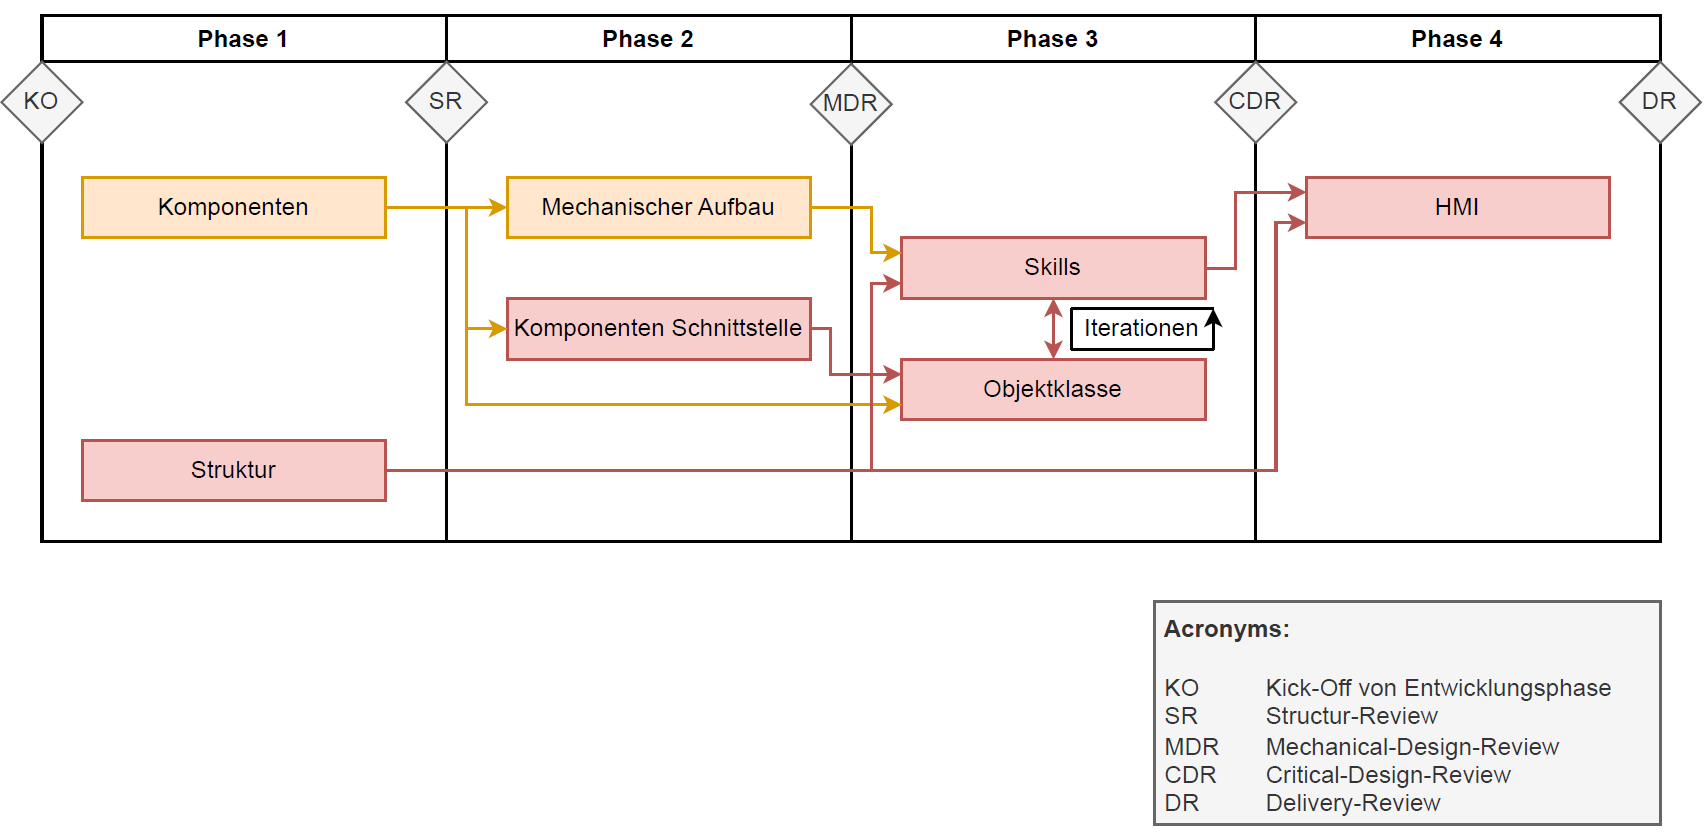
\includegraphics[width=1\textwidth]{03_Vorgehen_fuer_die_Thesis/Gateplan}
		\captionsetup{justification=centering}
		\caption{Definierter Gate-Plan}
		\label{fig:Gateplan}
	\end{figure}
	
	\textbf{Phase 1:} \vspace{2mm} 
	\\
		\begin{tabularx}{\textwidth}{@{}>{}p{7em} X@{}}
			Beschreibung: & 
			Phase 1 beschäftigt sich mit den Grundlagen der Hard- und Software. Die relevanten Komponenten müssen definiert und die notwendigen Fragen bezüglich der Software-Struktur geklärt werden.
			\\
			
			Output: & 
			\begin{itemize}
				\item Alle Komponenten für den Versuchsaufbau sind bekannt
				\item Die allgemeine Software-Struktur wurde definiert
			\end{itemize}
		\end{tabularx}
	
	\textbf{Phase 2:} \vspace{2mm} 
	\\
		\begin{tabularx}{\textwidth}{@{}>{}p{7em} X@{}}
			Beschreibung: & 
			Innerhalb von Phase 2 wird der Hardware-Teil abgeschlossen. Dafür wird der Versuchsaufbau konstruiert und gebaut. Zusätzlich werden die Software-Schnittstellen der Komponenten analysiert und definiert. 
			\\
			
			Output: & 
			\begin{itemize}
				\item Gebauter Versuchsbau für das Testen der Software
				\item Es ist bekannt, wie die Komponenten in die Software implementiert werden (in Theorie)
			\end{itemize}
		\end{tabularx}
	
	\textbf{Phase 3:} \vspace{2mm} 
	\\
		\begin{tabularx}{\textwidth}{@{}>{}p{7em} X@{}}
			Beschreibung: & 
			Phase 3 stellt die konkrete Umsetzung des skill-basierten Ansatzes in der Software dar. Hierbei wird iterativ die Software entwickelt. Die umfasst die Umsetzung der Struktur, wie auch die Entwicklung der Skills, der Objektklassen und des kompletten Prozessmodells.  
			\\
	
			Output: & 
			\begin{itemize}
				\item Funktionaler Prototyp, welcher an der Versuchsanlage getestet werden kann
			\end{itemize}
		\end{tabularx}
	
	\textbf{Phase 4:} \vspace{2mm} 
	\\
		\begin{tabularx}{\textwidth}{@{}>{}p{7em} X@{}}
			Beschreibung: & 
			Die letzte Phase beschäftigt sich mit der Entwicklung eines HMI.  
			\\
			
			Output: & 
			\begin{itemize}
				\item Über HMI bedienbarer Prototyp, welcher an der Versuchsanlage getestet werden kann
			\end{itemize}
		\end{tabularx}
	
	